% ============================================================
%  LLM-YARA: Structured LLM Pipeline for Automated YARA Rule
%  Generation — Full Technical Report
%  report source, 2026-03-17
% ============================================================
\documentclass[10pt,twocolumn]{article}

% ---------- geometry ----------
\usepackage[margin=0.75in]{geometry}

% ---------- fonts & encoding ----------
\usepackage[T1]{fontenc}
\usepackage[utf8]{inputenc}
\usepackage{lmodern}
\usepackage{microtype}

% ---------- maths ----------
\usepackage{amsmath,amssymb}

% ---------- tables ----------
\usepackage{booktabs}
\usepackage{multirow}
\usepackage{array}
\usepackage{tabularx}

% ---------- graphics ----------
\usepackage{graphicx}
\usepackage{xcolor}
\usepackage{float}
\usepackage[section]{placeins}
\usepackage{dblfloatfix}
\usepackage{tikz}
\usetikzlibrary{shapes.geometric, arrows.meta, positioning, fit, calc}
\usepackage{pgfplots}
\pgfplotsset{compat=1.18}

% ---------- code listings ----------
\usepackage{listings}
\lstset{
  basicstyle=\ttfamily\footnotesize,
  breaklines=true,
  columns=fullflexible,
  keepspaces=true,
  frame=single,
  numbers=left,
  numberstyle=\scriptsize\color{gray},
  keywordstyle=\color{blue!70!black}\bfseries,
  commentstyle=\color{green!50!black},
  stringstyle=\color{red!60!black},
  tabsize=4,
  captionpos=b
}

% ---------- hyperlinks & cross-refs ----------
\usepackage[colorlinks=true,linkcolor=blue!60!black,citecolor=blue!60!black,urlcolor=blue!60!black]{hyperref}
\usepackage[capitalise,noabbrev]{cleveref}

% ---------- captions ----------
\usepackage[font=small,labelfont=bf]{caption}

% ---------- misc ----------
\usepackage{enumitem}
\usepackage{xspace}
\usepackage{fancyhdr}

% ---------- compact spacing ----------
\setlength{\parskip}{0.4em}
\setlength{\parindent}{0em}
\setlength{\columnsep}{0.25in}
\raggedbottom

% ---------- short-hands ----------
\newcommand{\sysname}{\textsc{LLM-YARA}\xspace}
\newcommand{\topstrings}{\textsc{TopStrings}\xspace}
\newcommand{\apiary}{\textsc{Apiary-Static}\xspace}
\newcommand{\autoyara}{\textsc{AutoYara-Bicluster}\xspace}
\newcommand{\motif}{\textsc{MOTIF}\xspace}
\newcommand{\yamme}{\textsc{YAMME}\xspace}
\newcommand{\packgenome}{\textsc{PackGenome}\xspace}
\newcommand{\rulellm}{\textsc{RuleLLM}\xspace}

% ============================================================
\title{\textbf{LLM-YARA: A Structured LLM Pipeline for\\
Automated YARA Rule Generation}\\[4pt]
\large Final Technical Report}

\author{%
  Yassir BOUSSETA
}
\date{March 2026}
% ============================================================

\begin{document}
\maketitle
\thispagestyle{empty}

% ============================================================
\begin{abstract}
We present \sysname, a static-analysis-only pipeline that uses a
large language model (LLM) with structured generation and
deterministic rendering to produce YARA rules for malware family
detection.  Evaluated on 138 families from the \motif dataset under
identical train/test splits, \sysname achieves a mean~$F_1$ of
\textbf{0.4240} with a mean benign false-positive rate (FPR) of
\textbf{0.0\%} and mean rule specificity of \textbf{0.9988}.  This
represents a non-significant $F_1$ difference of $+0.0044$ ($p=0.85$)
relative to the \topstrings baseline (mean~$F_1=0.4195$), which
itself achieves higher recall (0.4797 vs.\ 0.4043) but lower
specificity (0.9924 vs.\ 0.9988).  The pipeline rejects 10 of 138
families through acceptance gates, yielding 128 accepted rules.  We
report all-family metrics as headline numbers and provide ok-only
figures as a secondary view.  Results are reported from saved
artifacts and checked once with replay.
\end{abstract}

% ============================================================
\section{Introduction}
\label{sec:intro}

YARA rules are a cornerstone of malware detection in operational
security workflows~\cite{yara2024}.  Analysts write rules that match
byte patterns, string literals, imports, and structural properties of
Portable Executable (PE) files to classify samples into malware
families.  Manual authoring of these rules does not scale: new families
emerge continuously, and maintaining high specificity across large
benign corpora is labor-intensive.

Automated YARA generation approaches have explored deterministic
string selection~\cite{autoyara2020}, static feature
heuristics~\cite{apiary2023ccs}, dynamic-trace
synthesis~\cite{yamme2023}, and packer-aware
pipelines~\cite{packgenome2023ccs}.  Recent work has also investigated
LLM-guided rule generation for intrusion detection
signatures~\cite{rulellm2025}.

This report describes \sysname, a pipeline that occupies a specific
point in the design space: \emph{static-only feature extraction},
\emph{structured primary LLM payloads},
\emph{deterministic rendering} of YARA syntax, and
\emph{acceptance gates} that reject rules failing minimum recall or
maximum FPR thresholds on held-out development data.

\textbf{Study question.}  Can a static-only LLM pipeline produce YARA
rules on the same split as deterministic baselines while keeping false
positives low?

We do not claim that \sysname beats \topstrings in $F_1$: the
difference is tiny and not statistically significant.  In this
evaluation, \sysname reaches mean $F_1=0.4240$, mean benign
FPR$=0.0000$, and 128 accepted families out of 138.

% ============================================================
\section{Dataset and Split Discipline}
\label{sec:dataset}

\subsection{The MOTIF Dataset}
We use the \motif malware reference dataset~\cite{joyce2022motif},
which provides ground-truth family labels for PE malware samples.
After filtering for families with at least 6~samples
(\texttt{min\_family\_size}=6), the evaluation covers \textbf{138
malware families}.

\subsection{Split Design}
All splits are deterministic (seed=42) and computed per-family:
\begin{itemize}[nosep,leftmargin=1.2em]
  \item \textbf{train\_target / test\_target}: 70\%/30\% of each
    family's samples (\texttt{test\_ratio}=0.3).
  \item \textbf{benign\_dev / benign\_test}: The benign corpus is
    split 60\%/40\% (\texttt{benign\_dev\_ratio}=0.6).
\end{itemize}

\textbf{Leakage prevention.}  LLM prompting uses
\texttt{train\_target} samples from the family under construction.
Feature selection ranks each family's \texttt{train\_target} positives
against \texttt{train\_other} plus \texttt{benign\_dev} negatives.
Final metrics are computed exclusively on \texttt{test\_target} and
\texttt{benign\_test}, which remain unseen during generation and final
scoring.  No baseline receives information from the test split.

% ============================================================
\section{System Design and Implementation}
\label{sec:design}

\sysname consists of six sequential stages, illustrated in
\cref{fig:pipeline}.

\begin{figure*}[t]
\centering
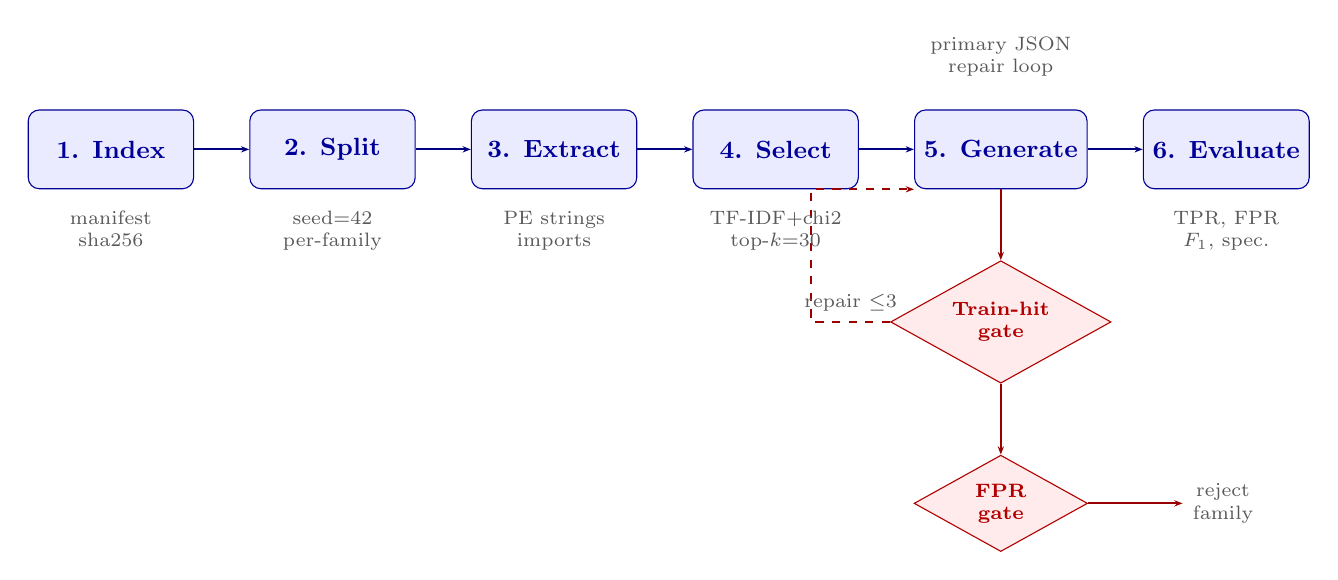
\begin{tikzpicture}[
  stage/.style={
    rectangle, rounded corners=4pt, draw=blue!60!black, fill=blue!8,
    minimum width=2.1cm, minimum height=1.0cm,
    font=\small\bfseries, text=blue!60!black, align=center
  },
  gate/.style={
    diamond, draw=red!70!black, fill=red!8,
    minimum width=1.2cm, minimum height=1.0cm,
    font=\scriptsize\bfseries, text=red!70!black, align=center,
    aspect=1.8
  },
  arr/.style={-{Stealth[length=3pt]}, thick, blue!50!black},
  garr/.style={-{Stealth[length=3pt]}, thick, red!60!black},
  note/.style={font=\scriptsize, text=gray!70!black, align=center},
]
  % Stages
  \node[stage] (idx) {1. Index};
  \node[stage, right=0.7cm of idx] (spl) {2. Split};
  \node[stage, right=0.7cm of spl] (ext) {3. Extract};
  \node[stage, right=0.7cm of ext] (sel) {4. Select};
  \node[stage, right=0.7cm of sel] (gen) {5. Generate};
  \node[stage, right=0.7cm of gen] (eva) {6. Evaluate};

  % Arrows between stages
  \draw[arr] (idx) -- (spl);
  \draw[arr] (spl) -- (ext);
  \draw[arr] (ext) -- (sel);
  \draw[arr] (sel) -- (gen);
  \draw[arr] (gen) -- (eva);

  % Gates inside generate
  \node[gate, below=0.9cm of gen] (g1) {Train-hit\\gate};
  \node[gate, below=0.9cm of g1]  (g2) {FPR\\gate};

  \draw[garr] (gen.south) -- (g1.north);
  \draw[garr] (g1.south)  -- (g2.north);

  % Repair loop
  \draw[garr, dashed] (g1.west) -- ++(-1.0,0)
    node[note, midway, above] {repair $\leq$3}
    |- (gen.south west);

  % Reject arrow
  \draw[garr] (g2.east) -- ++(1.2,0) node[note, right] {reject\\family};

  % Annotations
  \node[note, below=0.15cm of idx] {manifest\\sha256};
  \node[note, below=0.15cm of spl] {seed=42\\per-family};
  \node[note, below=0.15cm of ext] {PE strings\\imports};
  \node[note, below=0.15cm of sel] {TF-IDF+chi2\\top-$k$=30};
  \node[note, below=0.15cm of eva] {TPR, FPR\\$F_1$, spec.};

  % LLM callout
  \node[note, above=0.3cm of gen] {primary JSON\\repair loop};
\end{tikzpicture}
\caption{%
  \sysname pipeline.  Stages 1--4 are fully deterministic.
  Stage~5 queries the LLM for a structured JSON payload, renders
  YARA deterministically, and applies two acceptance gates.
  Stage~6 evaluates on the held-out test split.
}
\label{fig:pipeline}
\end{figure*}

\subsection{Stage 1: Index}
A manifest is built for every sample, recording its SHA-256 hash,
family label, data source, and file-system path.  This manifest anchors
all downstream references.

\subsection{Stage 2: Split}
Deterministic per-family stratified splitting produces
\texttt{train\_target} (70\%) and \texttt{test\_target} (30\%).  The
benign pool is split into \texttt{benign\_dev} (60\%) and
\texttt{benign\_test} (40\%).  All splits are seeded
(\texttt{seed}=42) for reproducibility.

\subsection{Stage 3: Extract}
Static PE features are extracted for every indexed sample: printable
ASCII and wide strings, PE import names (DLL and function), section
names, and PE metadata (timestamps, entry-point characteristics).  No
dynamic or behavioral features are used.

\subsection{Stage 4: Select}
Discriminative features are ranked with TF-IDF
vectorization~\cite{salton1988tfidf} and chi-squared scoring.  For each
family, the selector treats \texttt{train\_target} as positives and
\texttt{train\_other} plus \texttt{benign\_dev} as negatives.  The top
$k=30$ features per family are retained
(\texttt{top\_k\_features}=30).

\subsection{Stage 5: Generate}
\label{sec:generate}

The curated feature set is formatted into a structured prompt and sent
to the configured LLM backend (gpt-5-mini).  The model returns a
\textbf{JSON payload} specifying:
\begin{itemize}[nosep,leftmargin=1.2em]
  \item Selected string literals (up to \texttt{max\_strings}=20),
  \item Import predicates (DLL + function pairs),
  \item Section-based constraints,
  \item A condition skeleton (e.g., threshold count of string matches).
\end{itemize}

A \textbf{deterministic renderer} converts this JSON into syntactically
valid YARA source.  The primary generation path stays structured, while
repair payloads may preserve full YARA text returned by the model.

\textbf{Compile and repair.}  The rendered rule is compiled with
\texttt{yara-python}.  If compilation fails, the error message is fed
back to the LLM for a repair attempt, up to
\texttt{max\_repairs}=3.

\textbf{Train-hit gate.}  The compiled rule is scanned against
\texttt{train\_target}.  If fewer than \texttt{min\_train\_target\_hits}=1
sample matches, the family is rejected.

\textbf{Benign-dev FPR gate.}  The rule is scanned against
\texttt{benign\_dev}.  If the FPR exceeds
\texttt{benign\_dev\_fpr\_threshold}=0.02, the family is rejected.

\subsection{Stage 6: Evaluate}
Accepted rules are scanned against \texttt{test\_target} and
\texttt{benign\_test}.  Per-family metrics include: true positive rate
(TPR), false positive rate (FPR), $F_1$ score, rule specificity
($1 - \text{off-target rate}$), and rule complexity (string count plus
condition clause count).

\subsection{Implementation and Packaging}
The repository ships as a complete CLI workflow with
\path{Dockerfile}, \path{docker-compose.yml}, and \path{start.sh}.  The
default entrypoint validates the requested mode and required
dependencies before dispatching either a demo run or the full
index$\rightarrow$split$\rightarrow$extract$\rightarrow$select$\rightarrow$generate$\rightarrow$evaluate
pipeline.  Saved outputs under
\path{artifacts/final_motif_audit/} provide the numbers reported in this
document, while replay support allows a second pass over cached LLM
responses without changing the evaluation contract.

% ============================================================
\section{Experimental Protocol}
\label{sec:protocol}

\subsection{Headline vs.\ Secondary Metrics}
\textbf{All-family metrics} (138 families, failed families scored as
zero) are the headline results.  This penalizes \sysname for its 10
rejected families and prevents inflated numbers.
\textbf{Ok-only metrics} (128 accepted families) are reported
separately in \cref{app:okonly} as a secondary view of rule quality
among accepted families.

\subsection{Significance Testing}
Pairwise comparisons use a \textbf{paired randomization test} with
5,000 iterations and seed=42~\cite{noreen1989permutation}.  For each
pair of methods, per-family $F_1$ differences are randomly permuted to
build a null distribution.  A two-sided $p$-value below 0.05 is
required for significance.

\subsection{Configuration Summary}
\cref{tab:config} lists all pipeline parameters.

\begin{table}[h]
\centering
\caption{Pipeline configuration parameters.}
\label{tab:config}
\small
\begin{tabular}{@{}ll@{}}
\toprule
\textbf{Parameter} & \textbf{Value} \\
\midrule
\texttt{test\_ratio}             & 0.3   \\
\texttt{benign\_dev\_ratio}      & 0.6   \\
\texttt{min\_family\_size}       & 6     \\
\texttt{top\_k\_features}        & 30    \\
\texttt{max\_strings}            & 20    \\
\texttt{max\_repairs}            & 3     \\
\texttt{benign\_dev\_fpr\_threshold} & 0.02 \\
\texttt{min\_train\_target\_hits}    & 1    \\
\texttt{temperature\_config}      & 1.0   \\
\texttt{seed}                    & 42    \\
\texttt{model}                   & gpt-5-mini \\
\texttt{backend}                 & openai \\
\bottomrule
\end{tabular}
\end{table}

% ============================================================
\section{Executed Methods}
\label{sec:comparison}

Only methods executed within this repository appear in the main
comparison table.  \cref{tab:methods} lists each method and its
status.

\begin{table}[H]
\centering
\caption{Methods in the executed comparison set.}
\label{tab:methods}
\small
\begin{tabularx}{\columnwidth}{@{}llX@{}}
\toprule
\textbf{Method} & \textbf{Status} & \textbf{Note} \\
\midrule
\sysname           & Primary        & This work \\
\topstrings        & Reproduced     & Deterministic string baseline \\
\apiary            & Re-implemented & Static proxy of~\cite{apiary2023ccs} \\
\autoyara          & Re-implemented & Byte-$n$-gram biclustering \\
\bottomrule
\end{tabularx}
\end{table}

\yamme~\cite{yamme2023} and \packgenome~\cite{packgenome2023ccs} are
discussed in \cref{sec:related} as related work only.  Neither was
executed in this evaluation, and no numbers from those papers appear in
our comparison tables.  \rulellm~\cite{rulellm2025} informed the
structured-payload design but targets intrusion-detection signatures
rather than YARA rules.

% ============================================================
\section{Main Results}
\label{sec:results}

\cref{tab:main} presents all-family metrics across the four executed
methods.

\begin{table}[!b]
\centering
\caption{%
  Main comparison (all-family metrics, 138 families).
  Rejected families are scored as $F_1=0$, $\text{TPR}=0$.
  Best values per metric in \textbf{bold}; second-best \underline{underlined}.
}
\label{tab:main}
\scriptsize
\setlength{\tabcolsep}{3pt}
\begin{tabularx}{\columnwidth}{@{}Xcccccc@{}}
\toprule
\textbf{Method}
  & \textbf{OK}
  & \textbf{$F_1$}
  & \textbf{TPR}
  & \textbf{FPR\textsubscript{ben}}
  & \textbf{Spec.}
  & \textbf{Comp.} \\
\midrule
\sysname
  & 128\,/\,138
  & \textbf{0.4240}
  & 0.4043
  & \textbf{0.0000}
  & \textbf{0.9988}
  & 11.78 \\
\topstrings
  & \textbf{138\,/\,138}
  & \underline{0.4195}
  & \underline{0.4797}
  & 0.0061
  & \underline{0.9924}
  & \phantom{0}8.94 \\
\apiary
  & \textbf{138\,/\,138}
  & 0.1557
  & \textbf{0.6999}
  & 0.0718
  & 0.8638
  & \phantom{0}8.51 \\
\autoyara
  & \textbf{138\,/\,138}
  & 0.2760
  & 0.7965
  & 0.1183
  & 0.8180
  & 11.49 \\
\bottomrule
\end{tabularx}
\end{table}

\sysname has the numerically highest mean~$F_1$ (0.4240) and the highest
mean specificity (0.9988) with zero mean benign FPR.  However, the
$F_1$ difference from \topstrings is marginal: only $+0.0044$
absolute.

\smallskip
\noindent\textbf{Source: }\path{artifacts/final_motif_audit/comparison_summary.json}.

\topstrings delivers higher mean TPR (0.4797 vs.\ 0.4043) and covers
all 138 families.  Its specificity (0.9924) is lower than \sysname
but still high in absolute terms.

\apiary and \autoyara achieve substantially higher recall (0.6999 and
0.7965 respectively) but at the cost of high benign FPR (0.0718 and
0.1183) and much lower specificity (0.8638 and 0.8180), resulting in
lower $F_1$ scores.

Mean rule complexity for \sysname (11.78) is higher than \topstrings
(8.94) and \apiary (8.51), reflecting the multi-clause conditions
produced by the structured renderer (mean condition clause count of
2.21 vs.\ 1.0 for both baselines).  Mean string count is 9.57 for
\sysname vs.\ 7.94 for \topstrings.

\smallskip
\noindent\textbf{Example accepted rule.}  The Nanolocker family reaches
$F_1=1.0$, TPR$=1.0$, and benign FPR$=0.0$.  The saved rule combines a
PE header check, an import predicate, and thresholded string matching:

\begin{center}
\begin{minipage}{0.9\columnwidth}
\begin{lstlisting}[
  language={},
  basicstyle=\ttfamily\scriptsize,
  numbers=none,
  frame=single,
  xleftmargin=0pt,
  aboveskip=2pt,
  belowskip=2pt
]
strings:
  $a1 = "inet_addr" ascii
condition:
  uint16(0) == 0x5A4D and
  pe.imports("advapi32.dll",
             "abortsystemshutdowna") and
  1 of them
\end{lstlisting}
\end{minipage}
\end{center}

This snippet shows the final rule shape used by the primary method.
The full annotated rule remains in
\cref{app:rule}.  Source:
\path{outputs/final_motif_openai/rules/nanolocker.yar}.

% ============================================================
\section{Significance \& Trade-offs}
\label{sec:significance}

\subsection{Statistical Significance}

\cref{tab:sig} summarizes paired randomization test results.

\begin{table}[H]
\centering
\caption{Paired randomization tests (5,000 iterations, seed=42)
  comparing \sysname against each baseline on per-family $F_1$.}
\label{tab:sig}
\small
\begin{tabular}{@{}lccc@{}}
\toprule
\textbf{Comparison} & $\boldsymbol{\Delta F_1}$ & \textbf{$p$-value} & \textbf{Sig.?} \\
\midrule
vs.\ \topstrings & $+0.0044$ & 0.8484 & No  \\
vs.\ \apiary     & $+0.2683$ & 0.0002 & Yes \\
vs.\ \autoyara   & $+0.1480$ & 0.0002 & Yes \\
\bottomrule
\end{tabular}
\end{table}

The comparison with \topstrings is \textbf{not significant}
($p=0.85$).  The two methods are statistically tied on $F_1$.  The
differences against \apiary and \autoyara are highly significant
($p<0.001$).

\smallskip
\noindent\textbf{Source: }\path{artifacts/final_motif_audit/significance_vs_primary.json}.

\subsection{Trade-off Structure}
\label{sec:tradeoffs}

The four methods occupy distinct positions in the recall--specificity
trade-off space, visualized in \cref{fig:tradeoff}.

\begin{figure}[h]
\centering
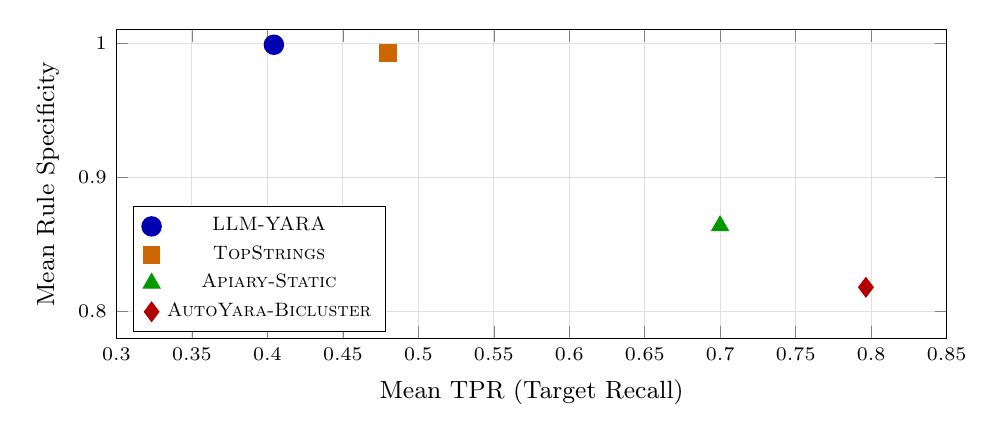
\begin{tikzpicture}
\begin{axis}[
  width=\columnwidth,
  height=5.5cm,
  xlabel={Mean TPR (Target Recall)},
  ylabel={Mean Rule Specificity},
  xmin=0.3, xmax=0.85,
  ymin=0.78, ymax=1.01,
  grid=major,
  grid style={gray!25},
  legend style={font=\scriptsize, at={(0.02,0.02)}, anchor=south west},
  every axis label/.style={font=\small},
  tick label style={font=\scriptsize},
]
  % LLM-YARA
  \addplot[only marks, mark=*, mark size=3.5pt, blue!70!black]
    coordinates {(0.4043, 0.9988)};
  \addlegendentry{\sysname}
  % TopStrings
  \addplot[only marks, mark=square*, mark size=3pt, orange!80!black]
    coordinates {(0.4797, 0.9924)};
  \addlegendentry{\topstrings}
  % Apiary
  \addplot[only marks, mark=triangle*, mark size=3.5pt, green!60!black]
    coordinates {(0.6999, 0.8638)};
  \addlegendentry{\apiary}
  % AutoYara
  \addplot[only marks, mark=diamond*, mark size=3.5pt, red!70!black]
    coordinates {(0.7965, 0.8180)};
  \addlegendentry{\autoyara}
\end{axis}
\end{tikzpicture}
\caption{%
  Recall--specificity trade-off.  \sysname occupies the
  high-specificity / lower-recall quadrant.  \autoyara and \apiary
  achieve higher recall at substantially lower specificity.
}
\label{fig:tradeoff}
\end{figure}

\sysname and \topstrings both occupy the high-specificity region, with
\sysname slightly higher on specificity and \topstrings slightly
higher on recall.  \apiary and \autoyara trade specificity for recall,
which reduces their $F_1$ due to high false-positive rates.

The clearest difference for \sysname is specificity: 0.9988 vs.\ 0.9924 for
\topstrings.  On this split, the lower benign FPR is the main reason
why \sysname remains numerically first on mean $F_1$ despite lower
recall.

% ============================================================
\section{Failure Analysis}
\label{sec:failures}

Of 138 families, \sysname rejects \textbf{10} through its acceptance
gates.  \cref{tab:failures_summary} categorizes these rejections.

\begin{table}[H]
\centering
\caption{Rejection reasons for the 10 failed families.}
\label{tab:failures_summary}
\small
\begin{tabular}{@{}lc@{}}
\toprule
\textbf{Rejection Reason} & \textbf{Count} \\
\midrule
\texttt{train\_target\_hits\_below\_min} & 7 \\
\texttt{benign\_dev\_fpr\_exceeded}      & 3 \\
\midrule
\textbf{Total rejected}                  & 10 \\
\bottomrule
\end{tabular}
\end{table}

\textbf{Train-hit failures (7 families):} Carbanak, Dridex,
MosaicRegressor, Nazar, Nymaim, Phorpiex, SmokeLoader.  These
families have samples where the LLM-selected features do not produce
rules matching even one training sample after up to 3 repair attempts.
Possible causes include packed or obfuscated samples where static
strings are absent, or families whose discriminative features are
behavioral rather than static.

\textbf{Benign-dev FPR failures (3 families):} Cerber, Dharma, Ryuk.
The generated rules match too many benign samples in
\texttt{benign\_dev}, exceeding the 0.02 FPR threshold.  This
suggests the LLM-selected features for these families overlap with
legitimate software patterns.

The 128/138 coverage gap (92.8\% family acceptance rate) is a
limitation.  All three baselines produce rules for all 138 families
because they lack acceptance gates.  However, those rules may have
high FPR (e.g., \autoyara achieves 0.1183 mean benign FPR across all
families).  The gate-based approach trades coverage for rule quality
assurance.

\smallskip
\noindent\textbf{Source: }\path{artifacts/final_motif_audit/failure_analysis.json}.

% ============================================================
\section{Related Work}
\label{sec:related}

\subsection{Executed Baselines}

\textbf{\topstrings.}  A deterministic baseline that selects the most
frequent family-discriminative strings and compiles them into a YARA
rule with a threshold condition.  Reproduced from scratch in our
repository and run on identical splits.

\textbf{\apiary}~\cite{apiary2023ccs} is treated here as
\textbf{literature-inspired static related work}.  We
\textbf{re-implemented a static proxy} (string/import discrimination)
to enable a controlled same-split comparison inside this repository.

\textbf{\autoyara}~\cite{autoyara2020} uses biclustering on byte
$n$-grams to identify common byte patterns across family members.  We
\textbf{re-implemented} the biclustering approach and evaluated it on
our splits.

\subsection{Cited-Only Methods}

\textbf{\yamme}~\cite{yamme2023} is cited as related work on automated
YARA generation.  It was not executed on this repository split, and
no numbers from \yamme appear in our comparison tables.

\textbf{\packgenome}~\cite{packgenome2023ccs} targets packed malware
by generating YARA rules from unpacking traces.  It addresses a
complementary problem (packer detection vs.\ family classification)
and was not executed in our evaluation.

\textbf{\rulellm}~\cite{rulellm2025} uses LLMs to generate Suricata
and Snort rules for network intrusion detection.  Its
structured-payload approach (LLM outputs a constrained schema rather
than freeform text) informed the design of our generation stage.
\rulellm targets network signatures, not YARA rules, and was not
benchmarked here.

% ============================================================
\section{Limitations and Conclusion}
\label{sec:conclusion}

\subsection{Limitations}

\textbf{Static-only scope.}  The pipeline extracts no dynamic,
behavioral, or network features.  Families whose distinguishing
characteristics are runtime behaviors (API call sequences, C2
communication patterns) may be poorly served.  The 7 train-hit
failures likely reflect this limitation.

\textbf{Tied with \topstrings on $F_1$.}  The $+0.0044$ $F_1$
difference is not statistically significant ($p=0.85$).  \topstrings
achieves higher recall (0.4797 vs.\ 0.4043) and covers all 138
families.  This favors \topstrings if recall and full coverage matter
more than benign FPR.

\textbf{Incomplete family coverage.}  Acceptance gates reject 10 of
138 families (7.2\%).  While this is a deliberate quality-control
mechanism, it means \sysname cannot produce rules for all families in
the dataset.

\textbf{LLM dependency.}  The pipeline requires API access to a
capable LLM.  Cost, latency, and model availability are practical
concerns.  Replay stays close to the primary run but is not bit-for-bit
identical, so exact equality should not be claimed.

\textbf{Single dataset.}  All results are on \motif.
Generalizability to other malware corpora, label sets, or PE
distributions is untested.

\subsection{Conclusion}

\sysname implements a structured LLM pipeline in which the model
selects features through a constrained JSON schema and a deterministic
renderer produces YARA syntax.

On \motif, the method reaches mean $F_1=0.4240$, mean benign
FPR$=0.0000$, mean specificity $=0.9988$, and accepted rules for
128 of 138 families.

The main observations are:
\begin{itemize}[nosep,leftmargin=1.2em]
  \item Numerically highest mean $F_1$ in the executed comparison, but not a
    significant difference from \topstrings.
  \item Zero benign FPR and the highest specificity among the four
    executed methods.
  \item Lower recall than \apiary and \autoyara, and 10 rejected
    families due to acceptance gates.
\end{itemize}

This method favors low false positives over recall and full family
coverage.

% ============================================================
% APPENDICES
% ============================================================
\clearpage
\onecolumn
\appendix

\section{Ok-Only Metrics}
\label{app:okonly}

\cref{tab:okonly} reports metrics computed only over the 128 families
for which \sysname produced accepted rules.  These numbers are
\textbf{not} the headline results; they characterize rule quality
among accepted families.

\begin{table}[h]
\centering
\caption{Ok-only metrics (128 accepted families for \sysname; all 138
  for baselines, whose ok-only equals all-family).}
\label{tab:okonly}
\small
\begin{tabular}{@{}lcccc@{}}
\toprule
\textbf{Method}
  & \textbf{Mean $F_1$}
  & \textbf{Mean TPR}
  & \textbf{Mean FPR\textsubscript{ben}}
  & \textbf{Mean Spec.} \\
\midrule
\sysname   & 0.4571 & 0.4359 & 0.0000 & 0.9987 \\
\topstrings & 0.4195 & 0.4797 & 0.0061 & 0.9924 \\
\apiary     & 0.1557 & 0.6999 & 0.0718 & 0.8638 \\
\autoyara   & 0.2760 & 0.7965 & 0.1183 & 0.8180 \\
\bottomrule
\end{tabular}
\end{table}

Among accepted families, \sysname mean~$F_1$ rises from 0.4240 to
0.4571.  This reflects the zero-score penalty imposed on the 10
rejected families in the all-family view.  Baselines have identical
ok-only and all-family numbers because they produce rules for all
families.

% ============================================================
\section{Significance Test Details}
\label{app:significance}

The paired randomization test proceeds as follows.

\textbf{Step 1.} For each of the $N=138$ families, compute the
per-family $F_1$ difference against a baseline:
\[
d_i = F_{1,i}^{(\text{\sysname})} - F_{1,i}^{(\text{baseline})}.
\]

\textbf{Step 2.} Compute the observed mean difference:
\[
\bar{d} = \frac{1}{N}\sum_i d_i.
\]

\textbf{Step 3.} For $B=5{,}000$ iterations (seed=42), randomly flip the
sign of each $d_i$ with probability 0.5 and recompute a permuted mean
difference $\bar{d}^{*}$.

\textbf{Step 4.} Estimate the two-sided $p$-value as:
\[
p = \frac{\left|\left\{ b : \left|\bar{d}^{*}_{b}\right| \geq \left|\bar{d}\right| \right\}\right|}{B}.
\]

Results:
\begin{itemize}[nosep,leftmargin=1.2em]
  \item \textbf{vs.\ \topstrings:}
    $\bar{d}=+0.004442$, $p=0.84843$. Not significant.
    The 138-family $F_1$ distributions of \sysname and \topstrings are
    statistically indistinguishable.
  \item \textbf{vs.\ \apiary:}
    $\bar{d}=+0.268289$, $p=0.0002$. Significant ($p<0.001$).
  \item \textbf{vs.\ \autoyara:}
    $\bar{d}=+0.147952$, $p=0.0002$. Significant ($p<0.001$).
\end{itemize}

% ============================================================
\section{Rejected Family List}
\label{app:rejected}

\cref{tab:rejected} lists all 10 families rejected by \sysname
acceptance gates.

\begin{table}[h]
\centering
\caption{Rejected families and rejection reasons.}
\label{tab:rejected}
\small
\begin{tabular}{@{}ll@{}}
\toprule
\textbf{Family} & \textbf{Rejection Reason} \\
\midrule
Carbanak        & \texttt{train\_target\_hits\_below\_min} \\
Dridex          & \texttt{train\_target\_hits\_below\_min} \\
MosaicRegressor & \texttt{train\_target\_hits\_below\_min} \\
Nazar           & \texttt{train\_target\_hits\_below\_min} \\
Nymaim          & \texttt{train\_target\_hits\_below\_min} \\
Phorpiex        & \texttt{train\_target\_hits\_below\_min} \\
SmokeLoader     & \texttt{train\_target\_hits\_below\_min} \\
\midrule
Cerber          & \texttt{benign\_dev\_fpr\_exceeded} \\
Dharma          & \texttt{benign\_dev\_fpr\_exceeded} \\
Ryuk            & \texttt{benign\_dev\_fpr\_exceeded} \\
\bottomrule
\end{tabular}
\end{table}

The train-hit failures cluster around families known for heavy
packing, polymorphism, or small static footprints.  The FPR failures
involve ransomware families (Cerber, Dharma, Ryuk) whose PE
characteristics may overlap with legitimate software (e.g., crypto
library imports, generic string patterns).

% ============================================================
\section{Annotated YARA Rule Example}
\label{app:rule}

\cref{lst:nanolocker} shows an excerpt of the \sysname-generated rule for the
Nanolocker family, which achieved perfect scores ($F_1=1.0$,
$\text{TPR}=1.0$, $\text{FPR}=0.0$, specificity=1.0, complexity=23).
The full rule text is taken from the saved primary output at
\texttt{outputs/final\_motif\_openai/rules/nanolocker.yar}.

\begin{lstlisting}[
  caption={Excerpt of the Nanolocker rule generated by \sysname.},
  label={lst:nanolocker},
  language={},
  morekeywords={import,rule,meta,strings,condition,uint16,and,of,them},
]
import "pe"
rule nanolocker_candidate_01 {
    meta:
        author = "automated-threat-detection"
        description = "High-signal substring candidates for Nanolocker"
        family = "nanolocker"
    strings:
        $a1 = "0a-%m]mm" ascii
        $a2 = "9j`mmlm" ascii
        $a3 = "mmm%m]mm" ascii
        $a4 = "mmmmmmmmmmmmmmmmh)m" ascii
        $a5 = "inet_addr" ascii
        $a6 = "2.83+?!" ascii
        $a7 = "\\mhavgco&" ascii
        $a8 = "cnr|*d\\1" ascii
        /* 12 additional strings omitted for readability */
    condition:
        uint16(0) == 0x5A4D and
        pe.imports("advapi32.dll", "abortsystemshutdowna") and
        1 of them
}
\end{lstlisting}

\textbf{Annotation.}  The rule combines three condition layers:
\begin{enumerate}[nosep,leftmargin=1.2em]
  \item \textbf{PE header check:} \texttt{uint16(0) == 0x5A4D}
    confirms the file is a PE binary.
  \item \textbf{Import predicate:}
    \texttt{pe.imports("advapi32.dll","abortsystemshutdowna")}
    targets a distinctive API import.  The
    \texttt{AbortSystemShutdownA} function is uncommon in legitimate
    software and characteristic of ransomware/locker families.
  \item \textbf{String matching:} \texttt{1 of them} requires at
    least one of the 20 string literals.  The strings are a mix of
    apparent binary-embedded data fragments (\$a1--\$a6) and
    higher-entropy substrings (\$a8--\$a20) selected by TF-IDF ranking.
\end{enumerate}

The combination of a rare import and multiple family-specific strings
yields high recall within the family while maintaining zero
false-positive rate against the benign test corpus.  Complexity is 23
(20 strings + 3 condition clauses), the highest among accepted rules,
but the multi-layer structure contributes directly to specificity.

% ============================================================
\section{Complexity and Rule Statistics}
\label{app:complexity}

\cref{tab:complexity} provides detailed rule-level statistics across
methods.

\begin{table}[h]
\centering
\caption{Rule complexity and size statistics (all-family means).}
\label{tab:complexity}
\small
\begin{tabular}{@{}lcccc@{}}
\toprule
\textbf{Method}
  & \textbf{Compl.}
  & \textbf{Strings}
  & \textbf{Cond.\ Cl.}
  & \textbf{Bytes} \\
\midrule
\sysname    & 11.78 & 9.57 & 2.21 & 655 \\
\topstrings & \phantom{0}8.94 & 7.94 & 1.00 & 582 \\
\apiary     & \phantom{0}8.51 & 7.51 & 1.00 & 568 \\
\autoyara   & 11.49 & 5.85 & 5.64 & 567 \\
\bottomrule
\end{tabular}
\end{table}

\sysname produces the most strings per rule (9.57) and a moderate
condition clause count (2.21), reflecting the structured renderer's
tendency to add PE header checks and import predicates alongside
string matches.  \autoyara has the highest condition clause count
(5.64) due to its biclustering-derived multi-clause conditions, but
fewer strings (5.85).  \topstrings and \apiary both use single-clause
conditions (threshold-based string matching) with moderate string
counts.

The mean rule size for \sysname (655~bytes) is the largest, driven by
longer string literals selected from TF-IDF features and additional
meta/import blocks.  This modest increase in rule size is acceptable
given the specificity gains.

\cref{fig:complexity_bar} visualizes the complexity breakdown.

\begin{figure}[h]
\centering
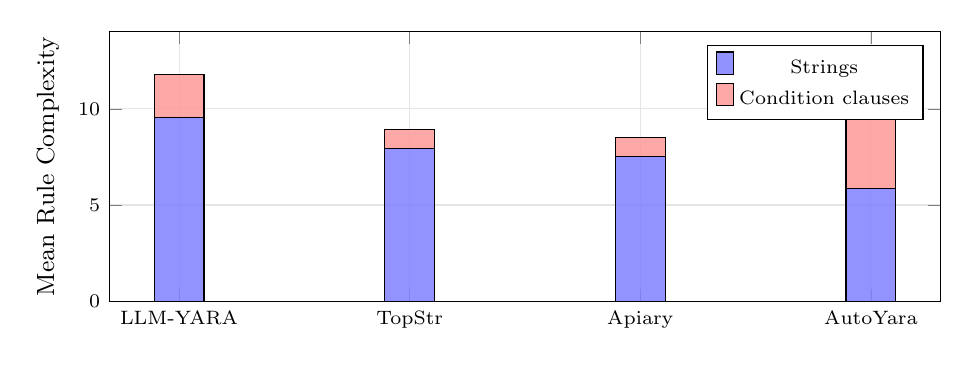
\begin{tikzpicture}
\begin{axis}[
  ybar stacked,
  width=\columnwidth,
  height=5cm,
  bar width=18pt,
  ymin=0, ymax=14,
  ylabel={Mean Rule Complexity},
  symbolic x coords={LLM-YARA, TopStr, Apiary, AutoYara},
  xtick=data,
  x tick label style={font=\scriptsize},
  y tick label style={font=\scriptsize},
  ylabel style={font=\small},
  legend style={font=\scriptsize, at={(0.98,0.95)}, anchor=north east},
  grid=major,
  grid style={gray!20},
  every axis plot/.append style={fill opacity=0.85},
]
  \addplot[fill=blue!50] coordinates
    {(LLM-YARA,9.57) (TopStr,7.94) (Apiary,7.51) (AutoYara,5.85)};
  \addlegendentry{Strings}
  \addplot[fill=red!40] coordinates
    {(LLM-YARA,2.21) (TopStr,1.00) (Apiary,1.00) (AutoYara,5.64)};
  \addlegendentry{Condition clauses}
\end{axis}
\end{tikzpicture}
\caption{Stacked complexity breakdown: string count plus condition clause count.}
\label{fig:complexity_bar}
\end{figure}

% ============================================================

\bibliographystyle{plain}
\bibliography{references}

\end{document}
